\documentclass[]{article}

%opening
\Huge\title{STAT 4352 - Mathematical Statistics Notes}
\Large\author{JaimeGoB}
\usepackage[margin=0.5in]{geometry}
\usepackage{physics}
\usepackage{amsmath}
\usepackage{centernot}
\usepackage{soul}
\usepackage{graphicx}
\graphicspath{ {../documentation/} }
\setul{}{1pt}

\begin{document}

\maketitle

\newpage
\Huge\section{Chapter 11 - Interval Estimation}
\Large\textbf{Point Estimators}
\newline $\theta$ is a unknown parameter (feature of a population)
\begin{itemize}
	\item Ex: population mean $\mu$
	\item \textbf{Fixed.} \newline
\end{itemize}
$\hat\theta$ is a point estimator of $\theta$ (it is a numerical value) 
\begin{itemize}
	\item Ex: sample mean $\bar{x}$
	\item \textbf{Varies from sample to sample.}
	\item No guarantee of \textul{accuracy}
	\item Must be \textit{supplemented by} Var($\theta$)
	\newline\Large\rule{1.3cm}{0pt} Standard Error SE($\hat\theta$) measures how much $\hat\theta$ varies from sample to sample.
	\newline\Large\rule{1.3cm}{0pt} small SE $\implies$ low variance thus a more reliable estimate of $\theta$ \newline
\end{itemize}
\Large\textbf{Interval Estimators} 
\newline
\newline\Large\textbf{Def: Interval Estimate}
\newline Provides a range of values that best describe the population.
\newline Let L = L(x) be the Lower Limit
\newline\Large\rule{0.68cm}{0pt} U = U(x) be the Upper Limit
\newline Both L,U are Random Variables because they are functions of sample data.
\newline
\newline\Large\textbf{Def: Confidence Level / Confidence Coefficient}
\newline Is the probability that the \textbf{interval estimate} will include population parameter $\theta$.
\begin{itemize}
	\item Sample means will follow the \textul{normal probability distribution} for large sample sizes (n $\ge$ 30)
	\item For small sample  forces us to use the \textul{t-distribution} probability distribution(n $<$ 30)
	\item \textul{A confidence level of 95$\%$} implies that \textbf{95$\%$ of all samples would give an interval that includes $\theta$, and only 5$\%$of all samples would yield an erroneous interval.}
	\item \textul{The most frequently used confidence levels are 90$\%$, 95$\%$, and 99$\%$ with corresponding Z-scores 1.645, 1.96, 2.576.}
	\item The higher the confidence level, the more strongly we believe that the value of the parameter lies within the interval.
\end{itemize}
\Large\textbf{Def: Confidence Interval}
\newline Gives plausible values for the parameter $\theta$ being estimated where degree of plausibility specified by a confidence level.
\newline
\newline To construct an interval estimator of unknown parameter $\theta$. We must find two statistics \textbf{L} and \textbf{U} such that:
 \[  P \{\textbf{L} \le \theta \le \textbf{U}  \}  = 1 - \alpha  \] 
\begin{itemize}
	\item $P \{\textbf{L} \le \theta \le \textbf{U} \}$ \textbf{Coverage Probability}, in repeated sampling, what percent of samples or Confident Intervals capture true $\theta$.
	\item 100(1- $\alpha$) \textbf{Confidence Interval }- for unknown fixed parameter $\theta$.
	\item L,U - \textbf{Lower and Upper Bounds} - RVs because they are functions of sample data. Vary from sample to sample.
	\item 1-$\alpha$ \textbf{Confidence Level} (Probability) estimate will include population parameter $\theta$.
	\item $\alpha$ \textbf{Level of Significance} Percent chance Confidence Interval will not contain population parameter $\theta$.
\end{itemize}
\Large\textbf{Def: Coverage Probability}
\newline $P \{\textbf{L} \le \theta \le \textbf{U} \}$ Gives what $\%$ of samples or Confidence Intervals capture true $\theta$.
\newline
\newline Ex: Coverage Probability = 95$\%$
\newline\Large\rule{1.3cm}{0pt} Will capture $\theta$, 95$\%$ of the time.
\newline\Large\rule{1.3cm}{0pt} Will NOT capture $\theta$, 5$\%$ of the time.
\newline
\newline\Large\textbf{Properties of Confidence Intervals}
\begin{itemize}
	\item Confidence Intervals are not unique.
	\item Desirable to have E[Length of CI] to be small.
	\item A one-sided 100(1-$\alpha$) lower-confidence interval on $\theta$:  L = -$\infty  \implies P\{ L \le \theta \} = 1-\alpha$
	\item A one-sided 100(1-$\alpha$) upper-confidence interval on $\theta$: $U = \infty  \implies P\{ \theta \le U \} = 1-\alpha$
	\item If L,U are both finite, then we have a two sided interval.
\end{itemize}
\Large\textbf{Correctly Interpreting Confidence Intervals}
\newline \textbf{Not Correct}
\newline There is 90$\%$ probability that the true population mean is within the interval.
\newline \textbf{Correct}
\newline There is a 90$\%$ probability that \textul{any given Confidence Interval from a random sample} will contain the true population mean.
\newline
\newline\textbf{How to Construct Confidence Interval Using Pivot Approach:} 
\newline Suppose we have a random sample X$_1$,X$_2$,...,X$_n$ from a population distribution and the parameter of interest is $\theta$.
\newline
\newline Given value $\alpha \in (0,1)$. We would like to construct a 1-$\alpha$ Confidence Interval using a Pivot Approach:
\begin{enumerate}
	\item\textbf{Find a variable Y, that is function of the parameter $\theta$ and data x.}
	\item\textbf{The distribution of newly created variable Y is free of $\theta$.}
\end{enumerate}
\textul{In many cases:}
\newline\Large\rule{3.0cm}{0pt}$Y = \dfrac{\hat{\theta} - \theta}{ SE(\hat{\theta})}$ is a pivot and the distribution of Y is symmetric about 0.
\newline
\newline
\newline\Large\textbf{ Using Pivot Approach for Two-Sided Intervals:}
\newline Find the critical points denoted c$_{\alpha \\/ 2}$ such that:
\[  P \{ -c_{\alpha \\/ 2} \le Y \le c_{\alpha \\/ 2}  \}   = 1 - \alpha  \] 
c$_{\alpha \\/ 2}$ is the upper ($\alpha$ / 2)100th percentile.
\newline
\newline \textbf{Critical points}- give you the area to the right of the point. \newline
\newline\textbf{Visualizing elements from Pivot Approach:}
\newline Let $\mu$ be parameter of interest. We can construct CI using pivot approach.
\newline
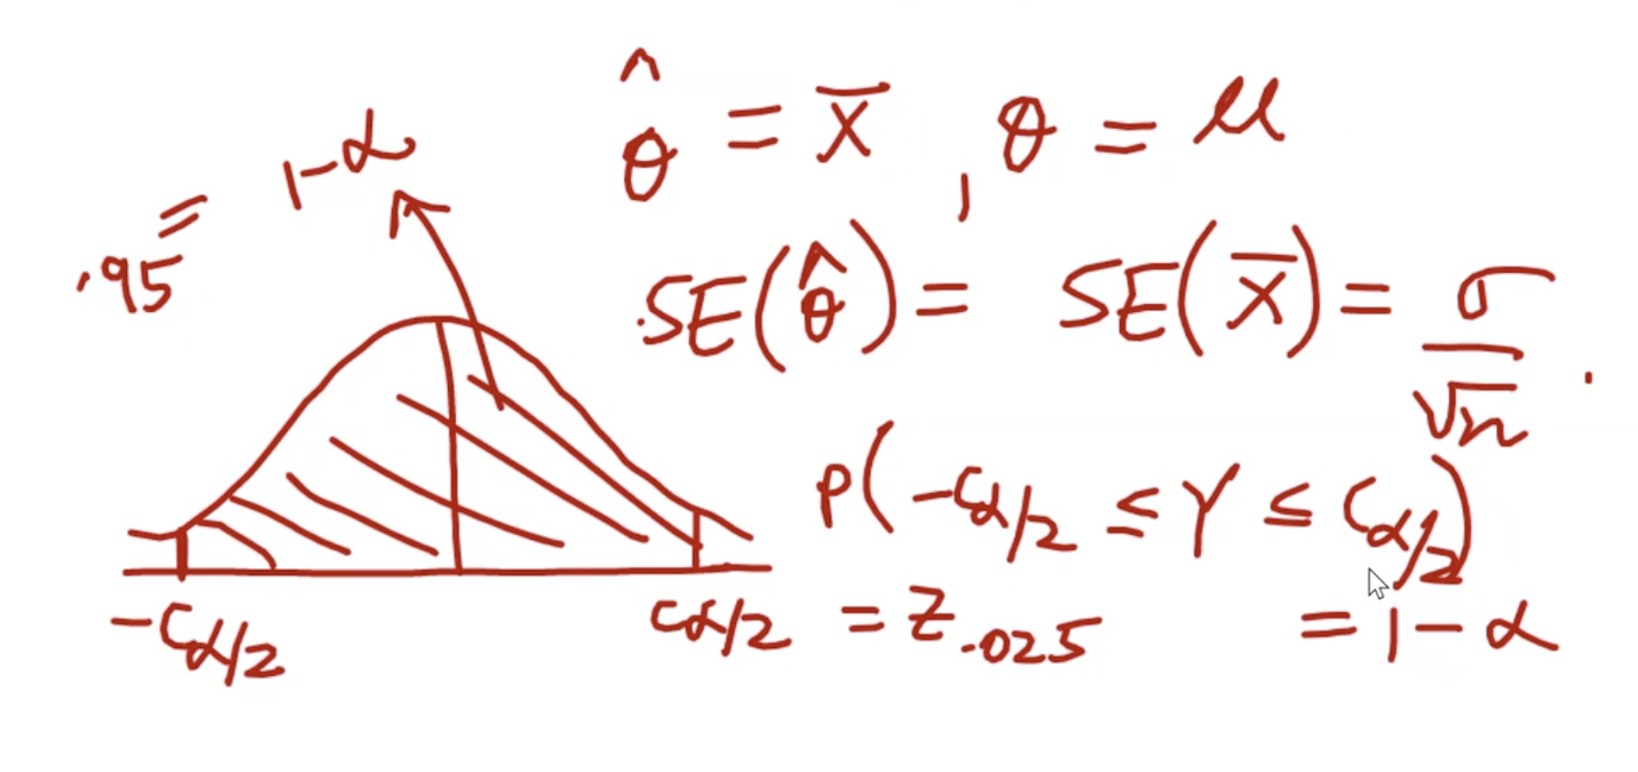
\includegraphics[scale=0.6]{general_ci_example}
\newline
\newline
\newline 
\newline
\Large\textbf{Symmetric Two-sided CI:}
\Large\textbf{Theorem}
\newline $ \hat\theta \pm c_{\alpha \\/ 2}(SE(\hat\theta))$ is a $100(1-\alpha)\%$ confidence interval for $\theta$
\newline 
\newline\Large\rule{3.0cm}{0pt} \textbf{Proof:}
\newline\Large\rule{3.0cm}{0pt}  $ 1 - \alpha =  P \{ -c_{\alpha \\/ 2} \le Y \le c_{\alpha \\/ 2}  \}$
\newline
\newline\Large\rule{4.3cm}{0pt}  $=  P \{ -c_{\alpha \\/ 2} \le \dfrac{\hat{\theta} - \theta}{ SE(\hat{\theta})}  \le c_{\alpha \\/ 2}  \}$
\newline
\newline\Large\rule{4.3cm}{0pt}  $=  P \{ \hat\theta -c_{\alpha \\/ 2} (SE(\hat\theta))  \le Y \le \hat\theta +c_{\alpha \\/ 2}(SE(\hat\theta))  \} $
\newline
\newline\Large\rule{4.3cm}{0pt} $\implies \hat\theta$ is \textbf{within} $c_{\alpha \\/ 2} (SE(\hat\theta))$ of $\theta$ with \textbf{probability}  1-$\alpha$
\newline
\newline $c_{\alpha \\/ 2} (SE(\hat\theta))$ is known as \textit{Margin of Error} (size of error in estimation)
\newline Ex: In polls you might hear accurate with 0.02 (this is margin of error)
\newline
\newline\Large\textbf{Asymmetric Two-sided CI(Non-symmetric distributions):}
\newline $[ \hat\theta - c_{\alpha \\/ 2}(SE(\hat\theta)),  \hat\theta - c_{1- \alpha \\/ 2}(SE(\hat\theta))]$ is a $100(1-\alpha)\%$ confidence interval for $\theta$
\newline 
\newline\Large\rule{3.0cm}{0pt} \textbf{Proof:}
\newline\Large\rule{3.0cm}{0pt}  $ 1 - \alpha =  P \{ c_{1- \alpha \\/ 2} \le Y \le c_{\alpha \\/ 2}  \}$
\newline
\newline\Large\rule{4.3cm}{0pt}  $=  P \{ c_{1- \alpha \\/ 2} \le \dfrac{\hat{\theta} - \theta}{ SE(\hat{\theta})}  \le c_{\alpha \\/ 2}  \}$
\newline
\newline\Large\rule{4.3cm}{0pt}  $=  P \{ \hat\theta - c_{\alpha \\/ 2}(SE(\hat\theta))  \le \theta \le \hat\theta - c_{1- \alpha \\/ 2}(SE(\hat\theta))  \} $
\newline\newline Ex: Chi-Square distribution critical points
\newline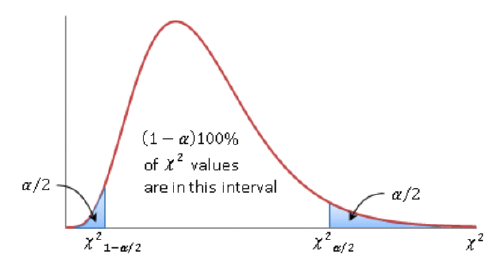
\includegraphics[scale=0.6]{assymetric_ci}
\newline
\newline
\newline
\newline
\newline
\Large\textbf{One-sided Confidence Bound:}
\newline A one-sided confidence bound defines the point where a certain percentage of the population is either higher or lower than the defined point.
\newline
\newline Upper Bound: U = $\hat\theta - c_{1- \alpha }(SE(\hat\theta))$ when  L = -$\infty$
\newline
\newline Lower Bound: L = $\hat\theta - c_{\alpha }(SE(\hat\theta))$ when  U = $\infty$
\newline
\newline\Large\rule{3.0cm}{0pt} \textbf{Proof(Upper Bound):}
\newline\Large\rule{3.0cm}{0pt} Coverage probability is 1 - $\alpha$.
\newline
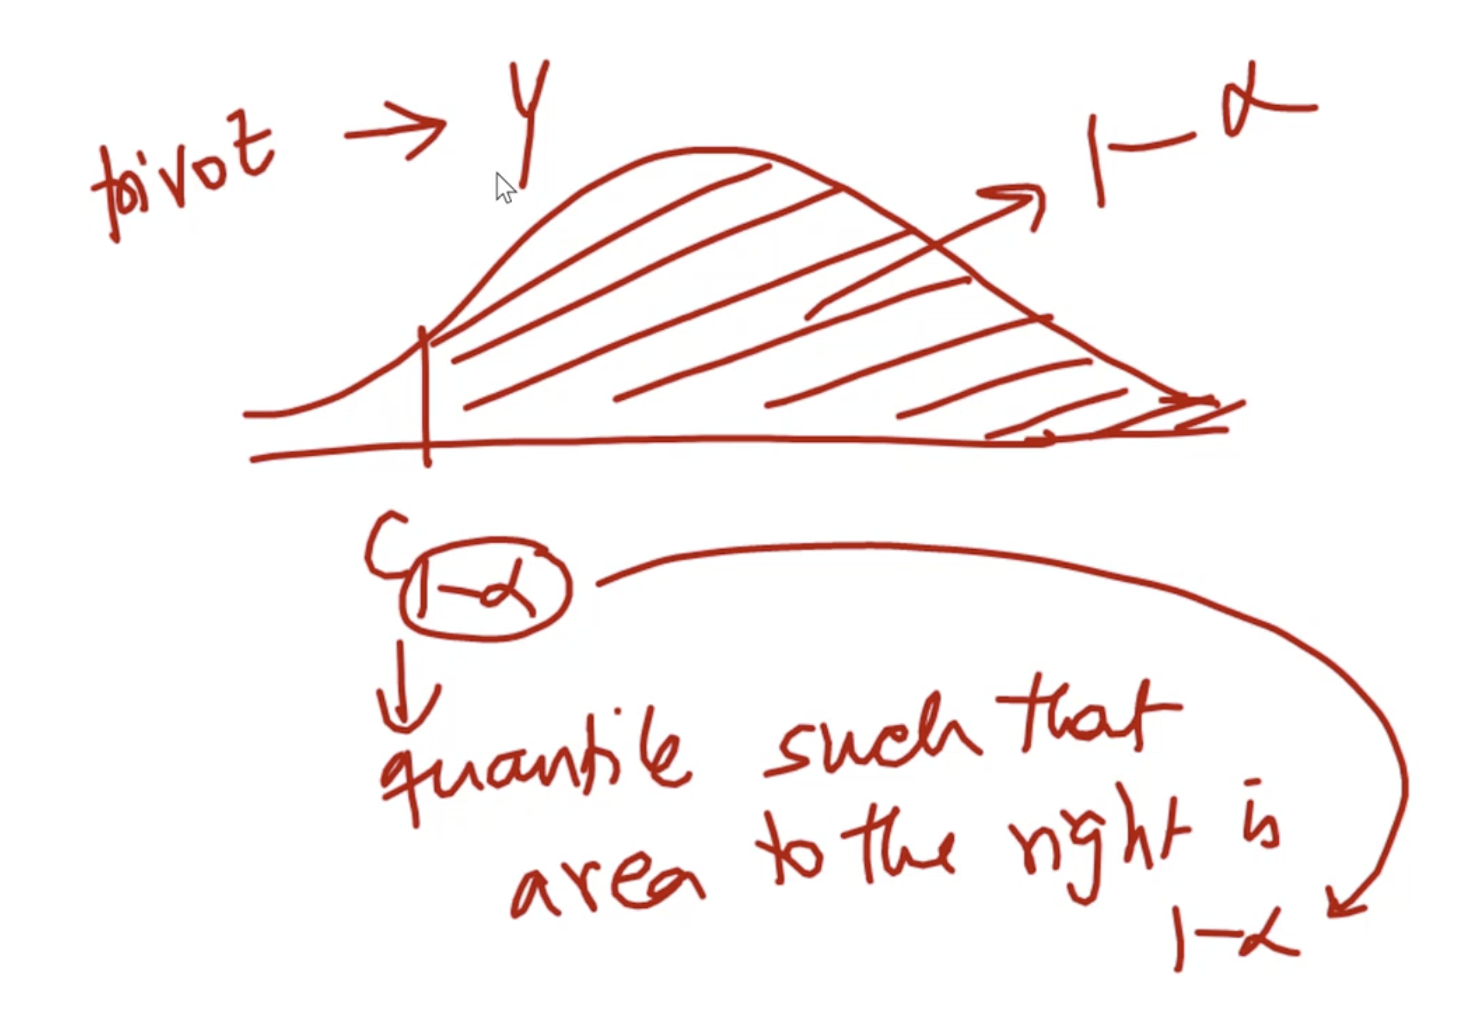
\includegraphics[scale=0.47]{one_sided_ci}
\newline\Large\rule{3.0cm}{0pt}  $ 1- \alpha =  P \{ Y \ge  c_{1- \alpha}  \}$
\newline
\newline\Large\rule{4.3cm}{0pt}  $=  P \{ \dfrac{\hat{\theta} - \theta}{ SE(\hat{\theta})}  \ge  c_{1- \alpha}   \}$
\newline
\newline\Large\rule{4.3cm}{0pt}  $=  P \{ \theta \le \hat{\theta} -  c_{1- \alpha }(SE(\hat\theta))  \}$
\newline
\newline\Large\rule{2.8cm}{0pt} $\implies$  U$=  \hat{\theta} -  c_{1- \alpha }(SE(\hat\theta))$
\newline The lower bound can be computed in the same manner.
\newline
\newline \textbf{How to interpret a one-sided CI?}
\newline For \textbf{Lower Bound} critical region $\in [ c_{\alpha} ,  \infty ]$:We are sure \textul{parameter $\theta$ is below} $c_{\alpha}$ 
\newline
\newline For \textbf{Upper Bound} critical region $\in [ - \infty , c_{1- \alpha} ]$:We are sure \textul{parameter $\theta$ is above} $c_{1- \alpha}$ 
\newline
\newline
\newline
\newline
\Large\textbf{Choice of Sample Size for CI for Mean when Variance Known }
\newline
\newline General form of a CI:
\newline 100(1-$\alpha$)$\%$ CI for $\theta$: $\hat{\theta} \pm c_{\alpha / 2} SE(\hat{\theta})$ 
\newline
\newline Mean $\mu$ of a Normal population: $\bar{x} \pm Z_{\alpha / 2 } \left( \dfrac{\sigma}{\sqrt{n}} \right)$
\newline \textbf{Margin Of Error:}  MOE = $Z_{\alpha / 2 } \left( \dfrac{\sigma}{\sqrt{n}} \right)$
\newline
\newline
\newline \textbf{Width of CI:} 2 $\times$ MOE = $2 \cdot Z_{\alpha / 2 } \left( \dfrac{\sigma}{\sqrt{n}} \right)$
\newline
\newline \textbf{Properties of MOE:} 
\begin{itemize}
	\item\textbf{As (1-$\alpha$) increases MOE increases:}
	\newline The larger the CI, the larger critical points are needed. 
	\newline As \textul{critical points increase,} Margin Of Error:  \textul{MOE} = $Z_{\alpha / 2 } \left( \dfrac{\sigma}{\sqrt{n}} \right)$ \textul{increase}
	\newline $\implies$ Increase in CI will make width of CI wider
	\item\textbf{As $\sigma$ increases MOE increases:}
	\newline
	\newline Margin Of Error: MOE = $Z_{\alpha / 2 } \left( \dfrac{\sigma}{\sqrt{n}} \right)$ \textul{$\sigma$ is part of numerator}, if it increases it will make \textul{MOE increase} too.
	\item\textbf{As \textit{n} increases MOE decreases:}
		\newline
	\newline Margin Of Error: MOE = $Z_{\alpha / 2 } \left( \dfrac{\sigma}{\sqrt{n}} \right)$ \textul{n is part of denominator}, if it increases it will make \textul{MOE decrease.}
	\newline
\end{itemize}
\textbf{Getting n from predefined MOE:} 
\newline Let E$_0$ be a pre-specified MOE. We can a value for n to make the following equation true.
\newline
\newline $\dfrac{Z_{\alpha / 2} \cdot \sigma}{\sqrt{n}}  \le E_0 $ solving for n we get: $n \ge \left( \dfrac{Z_{\alpha / 2} \cdot \sigma}{\sqrt{n} } \right)^2 $ (round up to nearest n.)
\newline
\newline We do this when we want to know how many observations (n) will give pre-specified margin of error - E$_0$
\newline
\newline
\newline
\newline
\Large\textbf{Theorem 11.1: Confidence Interval on the Mean of a Normal Distribution with known Variance}
\newline Let X be normal random variable with:
\newline\Large\rule{1.3cm}{0pt} Unknown mean $\mu$
\newline\Large\rule{1.3cm}{0pt} Known variance $\sigma ^2$
\newline Suppose a random sample n, ($X_1, X_2,...,X_n$) is taken.
\newline A 100(1-$\alpha$)$\%$ confidence interval on $\mu$ can be obtained by considering sampling distribution of the sample mean $\bar{X}$.
\newline
\newline\Large\rule{1.3cm}{0pt}\textbf{Central Limit Theorem:} 
\newline\Large\rule{1.3cm}{0pt} E($\bar{X}$) = $\mu$ and SD($\bar{X}$) = $\dfrac{\sigma}{\sqrt{n}}$, so $\bar{X} \sim \mathcal{N}(\mu, \dfrac{\sigma ^2}{ n })  $ as n$\to \infty$
\newline
\newline \Large\rule{1.3cm}{0pt} Let Z = Standardizing $\bar{X}$, Z will follow a Standard Normal Distribution
\newline 
\newline\Large\rule{1.3cm}{0pt} Let Z = $\dfrac{\bar{X} - \mu}{\sigma \\/ \sqrt{n} } \sim \mathcal{N}(0, 1) $
\newline 
\newline We can see from the image to the \textul{left:} \textbf{Distribution of Z} and the image to the \textul{right:} \textbf{Confidence Interval of 95$\%$}
\newline
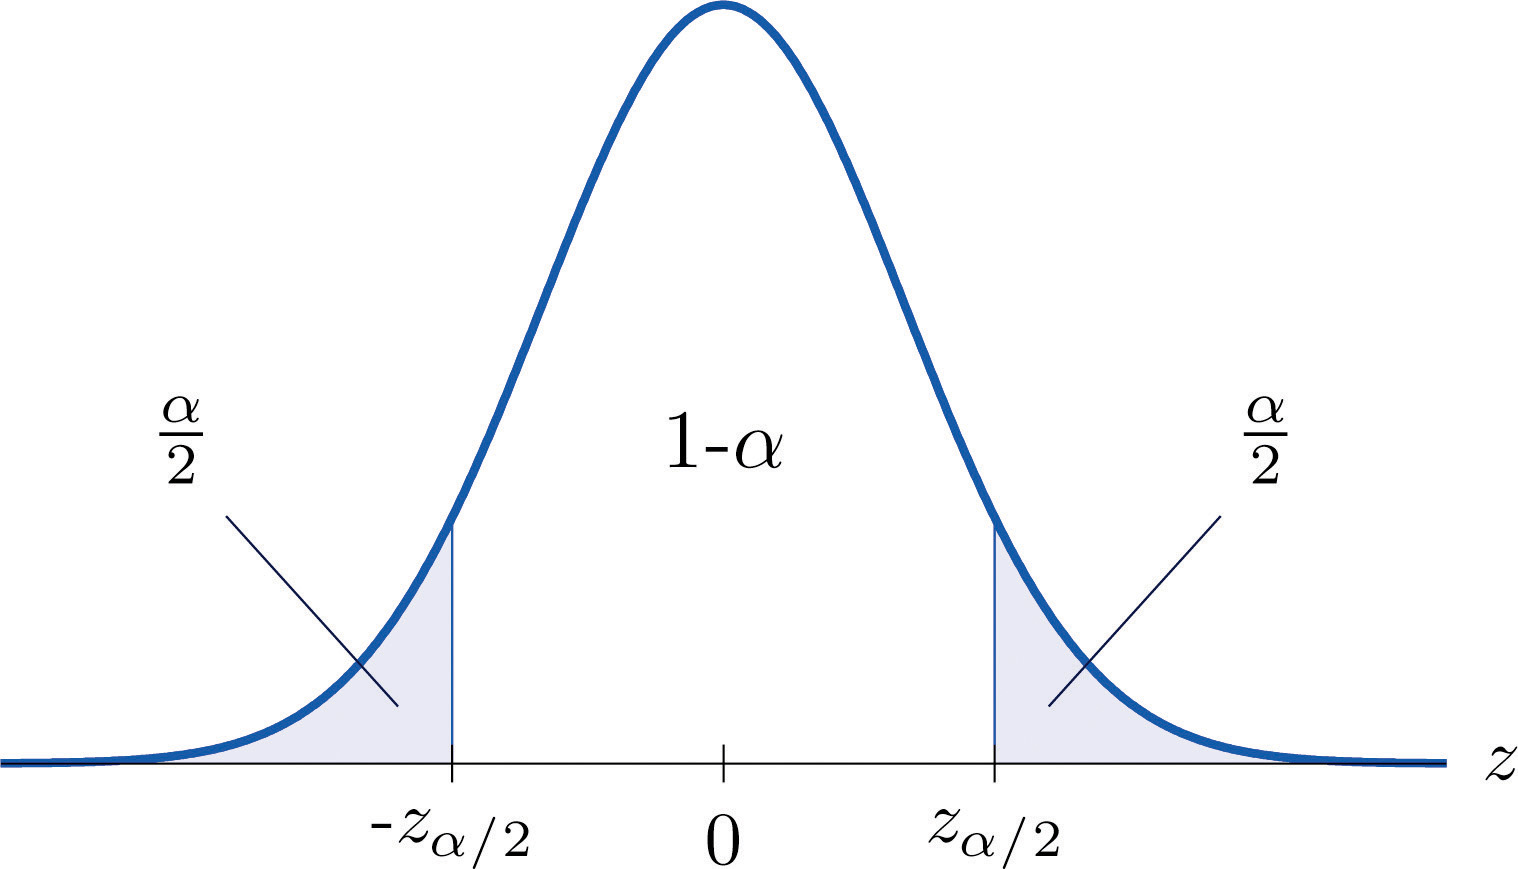
\includegraphics[scale=0.7]{distribution_of_Z}
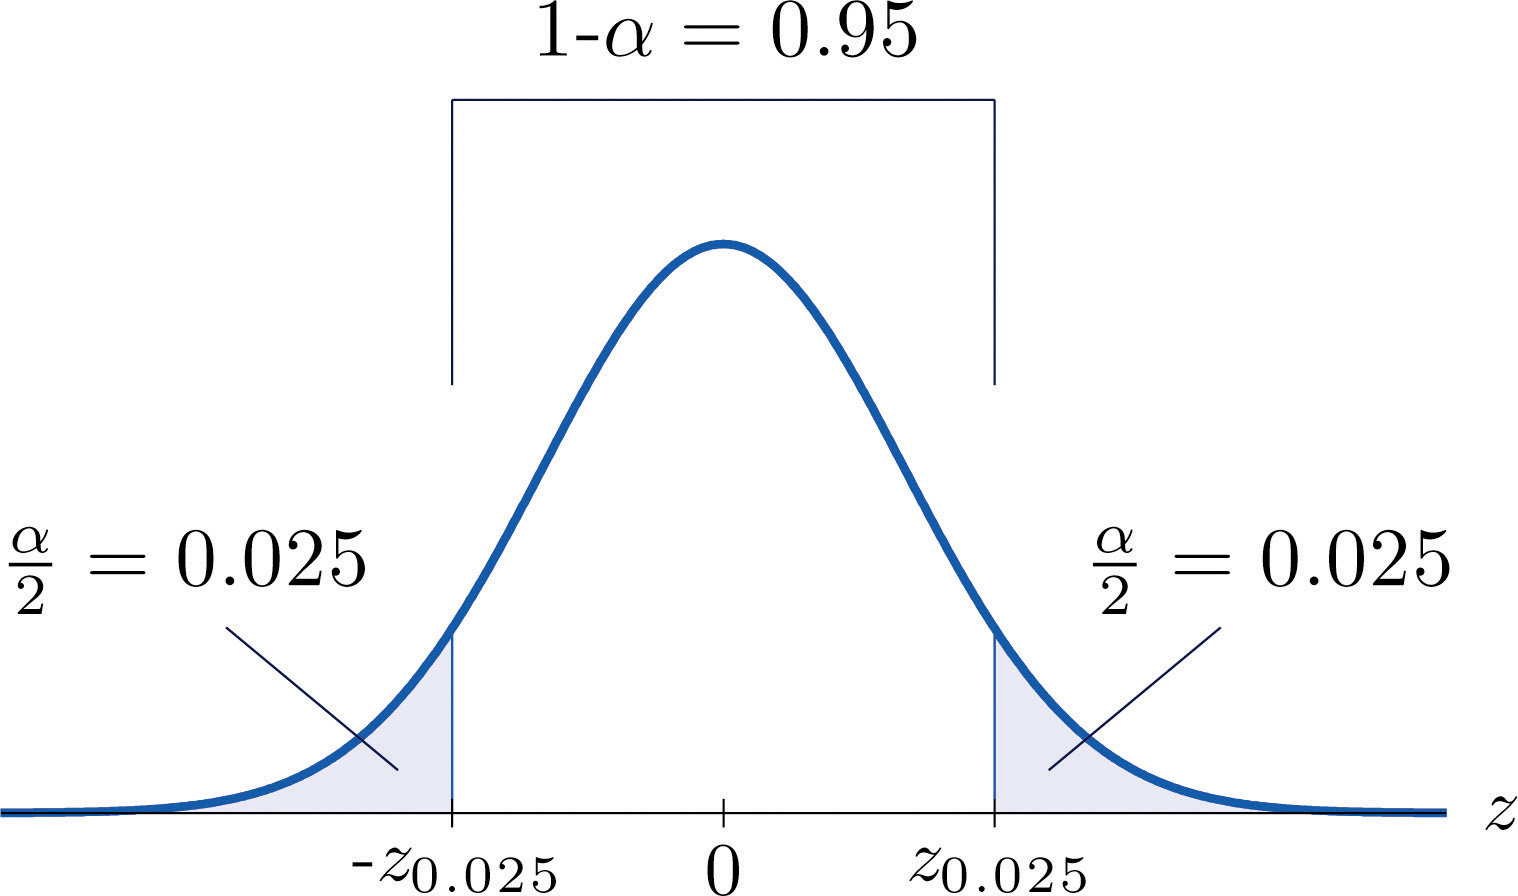
\includegraphics[scale=0.7]{ci_95}
\newline We can see that:
\newline 
\[  P \{ -Z_{\alpha\\/2} \le Z \le Z_{\alpha\\/2}  \}  = 1 - \alpha  \] 
\newline substituting Z into equation:
\[  P \{ -Z_{\alpha\\/2} \le \dfrac{\bar{X} - \mu}{\sigma \\/ \sqrt{n} }  \le Z_{\alpha\\/2}  \}  = 1 - \alpha  \] 
\newline isolating $\mu$:
\[  P \{ \bar{X}-Z_{\alpha\\/2} (\sigma \\/ \sqrt{n}) \le \mu \le \bar{X}+Z_{\alpha\\/2} (\sigma \\/ \sqrt{n})  \}   = 1 - \alpha  \] 
\newline Conclusion
$ \bar{X} \pm Z_{\alpha\\/2} (\sigma / \sqrt{n}) $ is a 100(1-$\alpha$)$\%$ CI for $\mu$ 
\newline
\Large\textbf{Confidence Interval on the Mean of a Normal Distribution
	\newline Variance Unknown and/or Small Sample:}
\newline
\newline $ \bar{X} \pm t_{n - 1, \alpha \\/ 2} \left(  \dfrac{s}{\sqrt{n}}  \right)$ is a $100(1-\alpha)\%$ CI for $\mu$
\newline
\newline\Large\rule{3.0cm}{0pt} \textbf{Proof:}
\newline\Large\rule{3.0cm}{0pt} We know that T = ${ \dfrac{\bar{X} - \mu}{ S \\/ \sqrt{n}}} \sim t_{n-1} $
\newline
\newline\Large\rule{3.0cm}{0pt}  $ 1- \alpha =  P \{ - t_{n - 1, \alpha \\/ 2} \le T \le t_{n - 1, \alpha \\/ 2}  \}$
\newline
\newline\Large\rule{4.3cm}{0pt}  $=  P \{ - t_{n - 1, \alpha \\/ 2} \le  \dfrac{\bar{X} - \mu}{ S \\/ \sqrt{n}}  \le t_{n - 1, \alpha \\/ 2}  \}$
\newline
\newline\Large\rule{4.3cm}{0pt}  $=  P \{ \bar{X}  - t_{n - 1, \alpha \\/ 2} (S \/ \sqrt{n})  \le \mu \le \bar{X} +  t_{n - 1, \alpha \\/ 2}( S \/ \sqrt{n})  \}$
\newline
\newline
\Large\textbf{Confidence Interval on the Mean no Specific Distribution \newline Variance Known}
\newline
\newline $ \bar{X} \pm Z_{\alpha\\/2} (\sigma / \sqrt{n}) $ is a 100(1-$\alpha$)$\%$ CI for $\mu$ 
\newline 
\newline\Large\rule{3.0cm}{0pt} \textbf{Proof:}
\newline\Large\rule{3.0cm}{0pt} Assuming the sample size is large (n $\ge$ 30) then by CLT:
\newline
\newline\Large\rule{3.0cm}{0pt}  Z = $\dfrac{\bar{X} - \mu}{\sigma \\/ \sqrt{n} } \sim N(0,1)$
\newline
\newline\Large\rule{3.0cm}{0pt} The mean of any distribution \textbf{provided} n is large (n $\ge$ 30) \newline\Large\rule{3.0cm}{0pt} can be approximated using a Normal Distribution.
\newline
\newline
\Large\textbf{Confidence Interval on the Mean no Specific Distribution \newline Variance Unknown}
\newline
\newline $ \bar{X} \pm Z_{\alpha\\/2} ( S / \sqrt{n}) $ is a 100(1-$\alpha$)$\%$ CI for $\mu$ 
\newline 
\newline\Large\rule{3.0cm}{0pt} \textbf{Proof:}
\newline\Large\rule{3.0cm}{0pt} Given the fact that S$^2$ is and unbiased estimator of $\sigma ^2$ we can
\newline\Large\rule{3.0cm}{0pt} \textul{use sample variance in lieu of population variance.} Also
\newline\Large\rule{3.0cm}{0pt}  sample size is large (n $\ge$ 30) then by CLT and LLN:
\newline
\newline\Large\rule{3.0cm}{0pt}  Z = $\dfrac{\bar{X} - \mu}{ S \\/ \sqrt{n} } = \dfrac{\bar{X} - \mu}{ \sigma \\/ \sqrt{n} } \left(\dfrac{\sigma}{S} \right) =  \dfrac{\bar{X} - \mu}{ \sigma \\/ \sqrt{n} } \sim N(0,1)$
\newline
\newline
\newline \Large\textbf{Confidence Interval on the Proportion of a Binomial Distribution}
\newline
\newline $\hat{p} \pm Z_{\alpha\\/2}\sqrt{\dfrac{\hat{p} (1-\hat{p} )}{n}} $ is a 100(1-$\alpha$)$\%$ CI for p 
\newline
\newline \textit{n} is random sample of size \textit{n} has been taken from a large population and X($\le n$) observations in this sample belong to a class of interest. 
\newline $\hat{p} = X/n$ is the point estimator of the proportion of the population that belongs to this class. 
\newline \textit{n} and p are the parameters of a binomial distribution.
\newline 
\newline\Large\rule{3.0cm}{0pt} \textbf{Proof:}
\newline\Large\rule{3.0cm}{0pt} The sampling distribution of $\hat{p}$ is approximately normal with mean p and 
\newline\Large\rule{3.0cm}{0pt} variance p(1-p)$/$n, if p is not too close to 0 or 1 and \textit{n} is large.
\newline
\newline\Large\rule{3.0cm}{0pt}  Z = $\dfrac{\hat{p} - p}{ \sqrt{\dfrac{p(1-p)}{n}}  } \sim N(0,1)$
\newline
\newline\Large\rule{3.0cm}{0pt} To construct CI on p, note that:
\newline
\newline\Large\rule{3.0cm}{0pt} $1 - \alpha \approx P \{ -Z_{\alpha\\/2} \le Z \le Z_{\alpha\\/2}  \}$
\newline
\newline\Large\rule{4.3cm}{0pt} $ \approx  P \{ -Z_{\alpha\\/2} \le \dfrac{\hat{p} - p}{ \sqrt{\dfrac{p(1-p)}{n}}  } \le Z_{\alpha\\/2}  \}$
\newline
\newline
\newline\Large\rule{4.3cm}{0pt} $ \approx  P \{\hat{p} - Z_{\alpha\\/2}\sqrt{\dfrac{p(1-p)}{n}}  \le p \le \hat{p} + Z_{\alpha\\/2}\sqrt{\dfrac{p(1-p)}{n}}   \}$
\newline
\newline\Large\rule{3.0cm}{0pt} Since the square root is the SE of estimator $\hat{p}$ and 
\newline\Large\rule{3.0cm}{0pt} also contains p in lower and upper bound.
\newline\Large\rule{3.0cm}{0pt} We can replace p with $\hat{p}$ and use Estimated SE instead of SE.
\newline
\newline\Large\rule{4.3cm}{0pt} $ \approx  P \{\hat{p} - Z_{\alpha\\/2}\sqrt{\dfrac{\hat{p} (1-\hat{p} )}{n}}  \le p \le \hat{p} + Z_{\alpha\\/2}\sqrt{\dfrac{\hat{p} (1-\hat{p} )}{n}}   \}$
\newline
\newline
\newline
\newline
\newline
\newline
\newline
\Large\textbf{Confidence Interval on the Variance or Standard Deviation of \newline a Normal Distribution - Mean is Unknown}
\newline
\newline
$\left[ \dfrac{(n-1)S^2}{\chi^{2}_{n-1,\alpha/2 }}, \dfrac{(n-1)S^2}{\chi^{2}_{n-1,1-\alpha/2 }} \right] $ is a 100(1-$\alpha$)$\%$ CI for $\sigma^2$ 
\newline 
\newline
\newline\Large\rule{3.0cm}{0pt} \textbf{Proof:}
\newline\Large\rule{3.0cm}{0pt} According to theorem 8.11:
\newline 
\newline\Large\rule{3.0cm}{0pt}  Y = $\dfrac{ \sum_{i=1}^{n} (x_i - \bar{x})^2  }{ \sigma^2 } = \dfrac{(n-1)S^2}{\sigma^2} \sim \chi^{2}_{n-1}$
\newline
\newline\Large\rule{3.0cm}{0pt} The critical points are: $\chi^{2}_{n-1,1-\alpha/2 }$ and $\chi^{2}_{n-1,\alpha/2 }$
\newline
\newline\Large\rule{3.0cm}{0pt} $1 - \alpha = P \{ \chi^{2}_{n-1,1-\alpha/2 } \le \dfrac{(n-1)S^2}{\sigma^2} \le \chi^{2}_{n-1,\alpha/2 } \} $
\newline
\newline\Large\rule{4.3cm}{0pt} $= P \left[  \dfrac{(n-1)S^2}{\chi^{2}_{n-1,\alpha/2 }}      \le   \sigma^2   \le  \dfrac{(n-1)S^2}{\chi^{2}_{n-1,1-\alpha/2 }}   \right]$
\newline 
\newline 
\Large\textbf{Confidence Interval on the Variance or Standard Deviation of \newline a Normal Distribution - Mean is Known}
\newline
\newline
$\left[ \dfrac{(n)S^2}{\chi^{2}_{n,\alpha/2 }}, \dfrac{(n)S^2}{\chi^{2}_{n,1-\alpha/2 }} \right] $ is a 100(1-$\alpha$)$\%$ CI for $\sigma^2$ 
\newline 
\newline
\newline\Large\rule{3.0cm}{0pt} \textbf{Proof:}
\newline\Large\rule{3.0cm}{0pt} Since $\mu$ is known then:
\newline\Large\rule{3.0cm}{0pt} Sum of n, squared standard normal distributions 
\newline\Large\rule{3.0cm}{0pt} $\implies$ Sum of n Chi-Square distributions with one df
\newline\Large\rule{3.0cm}{0pt} $\implies$ $\chi^{2}_{n}$
\newline 
\newline\Large\rule{3.0cm}{0pt}  Y = $\dfrac{ \sum_{i=1}^{n} (x_i - \mu )^2  }{ \sigma^2 } = \left( \dfrac{x_1 - \mu }{\sigma} \right) ^2 + ...+ \left( \dfrac{x_n - \mu }{\sigma} \right) ^2  \sim \chi^{2}_{n}$
\newline
\newline\Large\rule{3.0cm}{0pt} The critical points are: $\chi^{2}_{n,1-\alpha/2 }$ and $\chi^{2}_{n,\alpha/2 }$
\newline
\newline\Large\rule{3.0cm}{0pt} $1 - \alpha = P \{ \chi^{2}_{n,1-\alpha/2 } \le \dfrac{(n)S^2}{\sigma^2} \le \chi^{2}_{n,\alpha/2 } \} $
\newline
\newline\Large\rule{4.3cm}{0pt} $= P \left[  \dfrac{(n)S^2}{\chi^{2}_{n,\alpha/2 }}      \le   \sigma^2   \le  \dfrac{(n)S^2}{\chi^{2}_{n,1-\alpha/2 }}   \right]$
\newline 
\newline 
\Large\textbf{Two-Sample Confidence Interval Estimation}
\newline
\Large\textbf{Confidence Interval on the Difference between Means of Two Normal Distributions, Variances Known}
\newline In this case both \textul{means are unknown but variances are known.}
\newline
\newline
$\left[ \bar{X_{1}} - \bar{X_{2}} \pm \left( Z_{\alpha / 2}  \right) \sqrt{\dfrac{\sigma^2_1}{n_1} + \dfrac{\sigma^2_2}{n_2}    }      \right] $ is a 100(1-$\alpha$)$\%$ CI for $\mu_1 - \mu_2$ 
\newline 
\newline
\newline\Large\rule{3.0cm}{0pt} \textbf{Proof:}
\newline\Large\rule{3.0cm}{0pt} Let X$_1$ and X$_2$ be two normally distributed independent random variables.
\newline\Large\rule{3.0cm}{0pt} X$_1 \sim N( \mu_1, \sigma^2_1 )$  and X$_2 \sim N( \mu_2, \sigma^2_2 )$ 
\newline\Large\rule{3.0cm}{0pt} So, $\mu_1 - \mu_2 = \bar{X}_1 - \bar{X}_2$ $\implies$ SE($\bar{X}_1 - \bar{X}_2$) = SD($\bar{X}_1 - \bar{X}_2$) = $\sqrt{Var(\bar{X}_1 - \bar{X}_2 )}$
\newline\newline\Large\rule{3.0cm}{0pt} Because Var(A - B ) = Var(A) - Var(B) when A,B are independent
\newline\newline\Large\rule{3.0cm}{0pt} SE($\bar{X}_1 - \bar{X}_2$) = $\sqrt{\dfrac{\sigma^2_1}{n_1} + \dfrac{\sigma^2_2}{n_2} } \implies$   \fbox{$\bar{X}_1 - \bar{X}_2 \sim N(\bar{X}_1 - \bar{X}_2,\dfrac{\sigma^2_1}{n_1} + \dfrac{\sigma^2_2}{n_2}  )$} 
\newline\newline\Large\rule{3.0cm}{0pt} Independent random samples from normal populations:
\newline\newline\Large\rule{3.0cm}{0pt} Z = $\dfrac{  (  \bar{X}_1 - \bar{X}_2 )  -  (\mu_1 - \mu_2)   }{\sqrt{\dfrac{\sigma^2_1}{n_1} + \dfrac{\sigma^2_2}{n_2} }} \sim N(0,1)$
\newline\newline\Large\rule{3.0cm}{0pt}  Now, to construct a CI:
\newline
\newline\Large\rule{3.0cm}{0pt} $1 - \alpha = P \{ -Z_{\alpha\\/2} \le Z \le Z_{\alpha\\/2}  \}$
\newline
\newline\Large\rule{4.3cm}{0pt} $ = P \{ -Z_{\alpha\\/2} \le    \dfrac{  (  \bar{X}_1 - \bar{X}_2 )  -  (\mu_1 - \mu_2)   }{\sqrt{\dfrac{\sigma^2_1}{n_1} + \dfrac{\sigma^2_2}{n_2} }}    \le Z_{\alpha\\/2}  \}$
\newline
\newline
\newline\Large\rule{3.3cm}{0pt} $ = P \left[  (-Z_{\alpha\\/2} ) \sqrt{\dfrac{\sigma^2_1}{n_1} + \dfrac{\sigma^2_2}{n_2} }  \le  (  \bar{X}_1 - \bar{X}_2 )  -  (\mu_1 - \mu_2)  \le (Z_{\alpha\\/2}) \sqrt{\dfrac{\sigma^2_1}{n_1} + \dfrac{\sigma^2_2}{n_2} }  \right]$
\newline\newline
\newline\Large\rule{2.3cm}{0pt} $ = P \left[   \bar{X_{1}} - \bar{X_{2}} - \left( Z_{\alpha / 2}  \right) \sqrt{\dfrac{\sigma^2_1}{n_1} + \dfrac{\sigma^2_2}{n_2}    }  \le  \mu_1 - \mu_2    \le   \bar{X_{1}} - \bar{X_{2}} + \left( Z_{\alpha / 2}  \right) \sqrt{\dfrac{\sigma^2_1}{n_1} + \dfrac{\sigma^2_2}{n_2}    }  \right]$
\newline
\newline
\newline
\Large\textbf{Confidence Interval on the Difference between Means of Two Normal Distributions, Variances Unknown or Small Samples}
\newline Both \textul{means and variances are unknown.} However, we can assume $\sigma^2_1 = \sigma^2_2 =\sigma^2$
\newline
\newline
$\left[ \bar{X_{1}} - \bar{X_{2}} \pm \left( t_{n_{1}+ n_{2} -2 , \alpha / 2 }  \right) S_p \cdot  \sqrt{\dfrac{1}{n_1} + \dfrac{1}{n_2}    }      \right] $ is a 100(1-$\alpha$)$\%$ CI for $\mu_1 - \mu_2$ 
\newline 
\newline
\newline\Large\rule{3.0cm}{0pt} \textbf{Proof:}
\newline\Large\rule{3.0cm}{0pt} Let $S^2_1$ and $S^2_2$ be sample variances of random variables $X_1$ and $X_2$. Since 
\newline\Large\rule{3.0cm}{0pt} both sample variances are estimates of common variance $\sigma^2$ we can obtain
\newline\Large\rule{3.0cm}{0pt}  a  \textul{pooled estimator}  of $\sigma^2$.
\newline\Large\rule{3.0cm}{0pt} 
\newline\Large\rule{3.0cm}{0pt} $S^2_p = \dfrac{(n_1 -1)S^2_1 + (n_2 - 1) S^2_2}{n_2 + n_1- 2} \sim \chi^2_{n_1 -1} + \chi^2_{n_2 -1}$ 
\newline\newline\Large\rule{3.0cm}{0pt} Now pivot T
\newline\newline\Large\rule{3.0cm}{0pt} T = $\dfrac{  (  \bar{X}_1 - \bar{X}_2 )  -  (\mu_1 - \mu_2)   }{S_p \cdot \sqrt{\dfrac{1}{n_1} + \dfrac{1}{n_2} }} \sim t_{n_1 + n_2 - 2}$
\newline
\newline\newline\Large\rule{3.0cm}{0pt}  Now, to construct a CI:
\newline
\newline\Large\rule{3.0cm}{0pt} $1 - \alpha = P \{ -t_{n_1 + n_2 - 2, \alpha / 2} \le T \le t_{n_1 + n_2 - 2, \alpha /2} \}$ 
\newline
\newline
\newline\Large\rule{2.3cm}{0pt} $ = P \{ -t_{n_1 + n_2 - 2, \alpha / 2} \le \dfrac{ ( \bar{X}_1 - \bar{X}_  ) - (\mu_1 - \mu_2)   }{S_p \cdot \sqrt{\dfrac{1}{n_1} + \dfrac{1}{n_2} }} \le t_{n_1 + n_2 - 2, \alpha /2} \}$
\newline
\newline
\newline
$P \left[  -t_{n_1 + n_2 - 2, \alpha / 2} \left( S_p \cdot \sqrt{\dfrac{1}{n_1} + \dfrac{1}{n_2}} \right) \le  (  \bar{X}_1 - \bar{X}_2 )  -  (\mu_1 - \mu_2) \le t_{n_1 + n_2 - 2, \alpha /2} \left( S_p \cdot \sqrt{\dfrac{1}{n_1} + \dfrac{1}{n_2}} \right)  \right]$
\newline
\newline
\newline After solving for both population means:
\newline
\newline$P\left[  \bar{X}_1 - \bar{X}_2 - ( t_{n_1 + n_2 - 2, \alpha / 2} ) S_p \sqrt{\dfrac{1}{n_1} + \dfrac{1}{n_2}}  \le  \mu_1 - \mu_2 \le  \bar{X}_1 - \bar{X}_2  +  (t_{n_1 + n_2 - 2, \alpha /2}) S_p \sqrt{\dfrac{1}{n_1} + \dfrac{1}{n_2}} \right]$
\newline
\newline\newline\newline
\newline
\Large\textbf{Confidence Interval on the Difference between Means of Two Normal Distributions, Variances Unknown and Variances Differ}
\newline Both \textul{means and variances are unknown and the variances are not equal} $\sigma^2_1 \ne \sigma^2_2$. In this case we make the assumption that variances are different.
\newline
\newline
$\left[ \bar{X_{1}} - \bar{X_{2}} \pm \left( t_{v, \alpha / 2 }  \right) \sqrt{\dfrac{S^2_1}{n_1} + \dfrac{S^2_2}{n_2}    }      \right] $ is a 100(1-$\alpha$)$\%$ CI for $\mu_1 - \mu_2$ 
\newline 
\newline
\newline\Large\rule{3.0cm}{0pt} \textbf{Proof:}
\newline\Large\rule{3.0cm}{0pt} From previous cases we know that:
\newline\Large\rule{3.0cm}{0pt}   \fbox{$\bar{X}_1 - \bar{X}_2 \sim N(\bar{X}_1 - \bar{X}_2,\dfrac{\sigma^2_1}{n_1} + \dfrac{\sigma^2_2}{n_2}  )$}  
\newline\newline\Large\rule{3.0cm}{0pt} Now let Y be the \textul{approximate} pivot:
\newline\newline\Large\rule{3.0cm}{0pt} T = $\dfrac{  (  \bar{X}_1 - \bar{X}_2 )  -  (\mu_1 - \mu_2)   }{\sqrt{\dfrac{S^2_1}{n_1} + \dfrac{S^2_2}{n_2}}} \approx t_{v}$ 
where df
v = $\dfrac{  (  S^2_1 / n_1  + S^2_2 / n_2  )^2  }{  \dfrac{(S^2_1 / n_1)^2}{n_1 +1}   +  \dfrac{(S^2_2 / n_2)^2}{n_2 +1}    }$
\newline
\newline 
\newline\Large\rule{3.0cm}{0pt} $1 - \alpha = P \{ -t_{v, \alpha / 2} \le T \le t_{v, \alpha / 2} \}$ 
\newline
\newline
\newline\Large\rule{4.3cm}{0pt} $ = P \{ -t_{v, \alpha / 2} \le \dfrac{  (  \bar{X}_1 - \bar{X}_2 )  -  (\mu_1 - \mu_2)   }{\sqrt{\dfrac{S^2_1}{n_1} + \dfrac{S^2_2}{n_2}}}  \le t_{v, \alpha /2} \}$
\newline
\newline
\newline
$P \left[  -t_{v, \alpha / 2} \left( \sqrt{\dfrac{S^2_1}{n_1} + \dfrac{S^2_2}{n_2}} \right) \le  (  \bar{X}_1 - \bar{X}_2 )  -  (\mu_1 - \mu_2) \le t_{v, \alpha /2} \left( \sqrt{\dfrac{S^2_1}{n_1} + \dfrac{S^2_2}{n_2}} \right)  \right]$
\newline
\newline
\newline After solving for both population means:
\newline
\newline$P \left[ \bar{X}_1 - \bar{X}_2 - ( t_{v, \alpha / 2} )  \sqrt{\dfrac{S^2_1}{n_1} + \dfrac{S^2_2}{n_2}}  \le  \mu_1 - \mu_2 \le \bar{X}_1 - \bar{X}_2  + ( t_{v, \alpha /2} ) \sqrt{\dfrac{S^2_1}{n_1} + \dfrac{S^2_2}{n_2}}  \right]$
\newline 
\newline
\newline 
\newline
\newline 
\newline\Large\textbf{Confidence Interval on the Ratio of Variances of Two Normal Distributions}
\newline
\newline
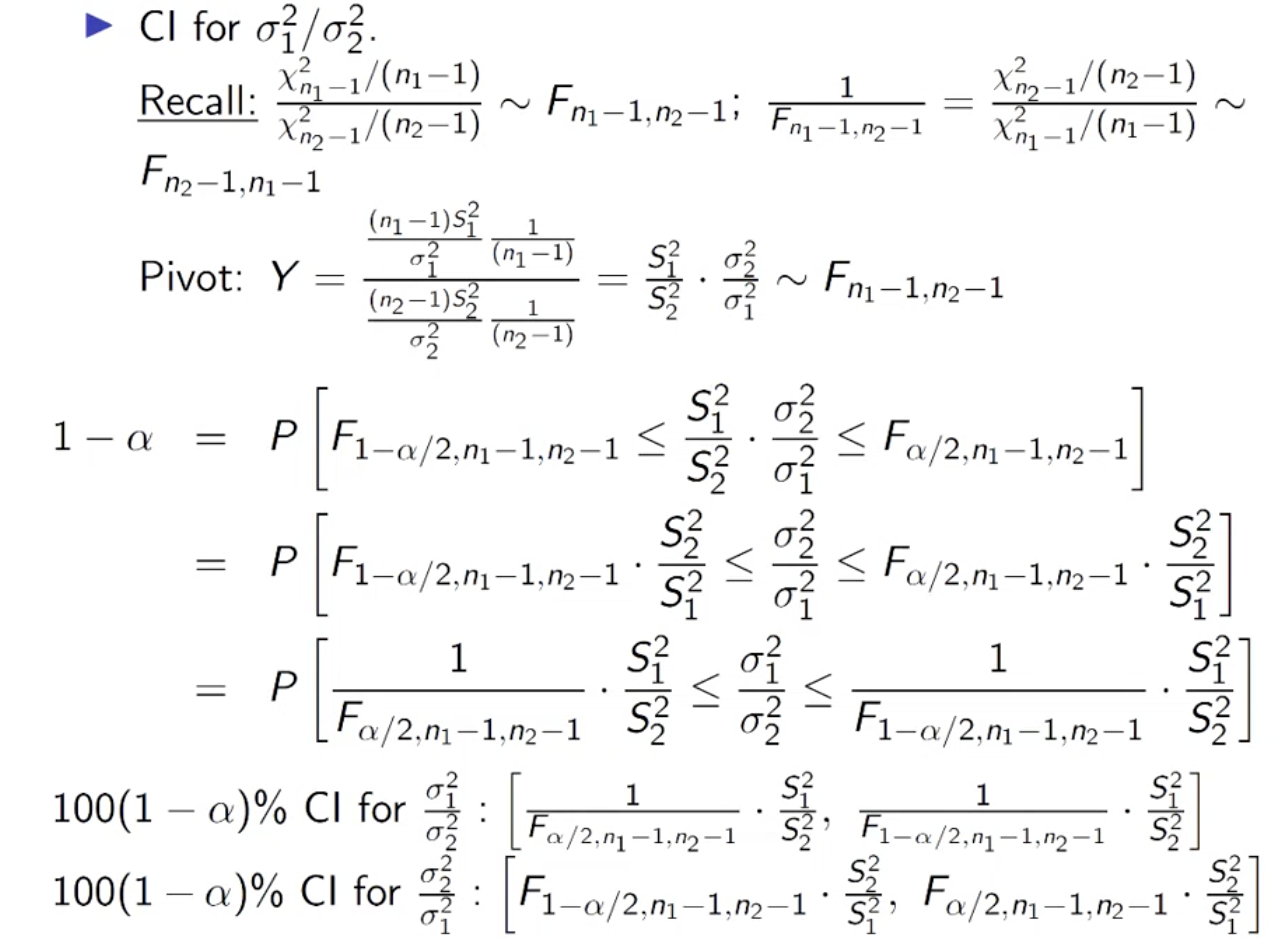
\includegraphics[scale=0.8]{ratio_of_variances}
%\Large\rule{2.3cm}{0pt} \textbf{fixed}
 %\textbf{(Unbiased Estimator)}\newline
 
\section{}

\end{document}












